\documentclass[conference]{IEEEtran}
\IEEEoverridecommandlockouts
\usepackage[T1]{fontenc}
\usepackage{amsmath,amssymb}
\usepackage{graphicx}
\usepackage{booktabs}
\usepackage{array}
\usepackage{microtype}
\usepackage[table]{xcolor}
\usepackage{cite}
\usepackage[hidelinks]{hyperref}

\newcommand{\pp}{\,pp}
\newcommand{\todo}[1]{\textbf{[TODO: #1]}}
\graphicspath{{figures/}}

\begin{document}

\title{An Audited, Budget-Disclosed Benchmark of Classical Teachers\\and Learned Students on a Simulated Arm}

\author{\IEEEauthorblockN{Hao-Ting Ho}
\IEEEauthorblockA{Department of Electrical Engineering, Tunghai University\\
Taichung, Taiwan\\
haoting.ho@outlook.com}}

\maketitle

\begin{abstract}
Learned-versus-classical comparisons rarely give the classical side comparable tuning, a disclosed budget, and rules fixed before testing. We propose an audited protocol for simulated arm control: tuned classical baselines, budgets disclosed on three axes (episodes, wall-clock, label source), rules time-stamped before testing, a sanity gate (a learner must first learn a known-learnable correction), and a test-evaluation log. Across 8 tracking, juggling and whip settings, no learned method cleared the pre-specified +10 percentage-point (pp) bar over the strongest classical baseline, and only whip was measured to leave room. In 3 settings the residual reinforcement-learning (RL) learner did not learn; in two of them (juggling and idealised whip), with a gate-passing exploration scale, it degraded its base (its classical start) by 17.6--23.8\pp. On realistic whip, a once-only set, TEST-C ($n{=}500$), shows that the true physical parameters add +17.6\pp\ [12.6, 22.6]. Robust plan selection scores candidate swings under several plausible parameter sets; it was built for the learned side and then given to the classical side. On a second such set, TEST-D (gap +18.0\pp), it alone recovers 0.59 [0.36, 0.82] of the gap with a classical ensemble, and 0.90 [0.68, 1.16] when combined with estimators trained on simulator labels and true-plant oracle plans. The learned side leads by +5.6\pp\ [0.6, 10.6]; 10\pp\ cannot be excluded. One simulator, mostly one task.
\end{abstract}

\begin{IEEEkeywords}
robot manipulation, classical versus learned control, imitation learning, residual reinforcement learning, evaluation protocol, whip
\end{IEEEkeywords}

\section{Introduction}
\label{sec:intro}

\begin{figure*}[t]
\centering
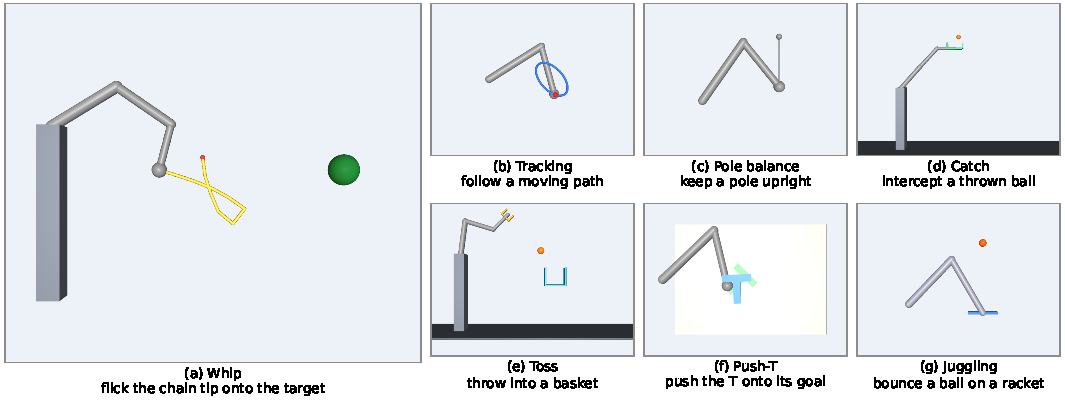
\includegraphics[width=\textwidth]{fig_tasks}
\caption{The seven tasks use planar MuJoCo arms (two links by default, three for whip). Each panel is a MuJoCo render under nominal parameters, taken from a classical teacher's rollout on a calibration seed. Whip (a), the main test bed, must flick a passive chain so that its tip hits the target. Script: \texttt{figures/make\_task\_renders.py}.}
\label{fig:tasks}
\end{figure*}

Claims that a learned controller beats a classical one steer which methods researchers pursue and which ones practitioners deploy, so the comparison behind such a claim has to hold up. It is often weaker than it looks, and our own first experiment shows how. A residual policy (a learned correction added to the classical controller's command), trained with proximal policy optimisation (PPO), beat the untuned computed-torque teacher on a 2-DoF tracking task by 16.7\% in root-mean-square tracking error (RMSE) without disturbances. After a two-parameter gain retune of the teacher, the advantage disappeared: the learned side was 7.1\% worse, with a 95\% confidence interval (CI) of $[-13.8, +0.3]\%$ (setting S1 in Table~\ref{tab:cross}). The gap was a tuning gap, not a learning gap.

This paper asks a narrower question than ``does learning win'': \emph{what extra ingredient does a learned student need to beat its classical teacher?} Candidate ingredients are more information (privileged state), better optimisation (reinforcement learning, RL, on top of the teacher), a richer model class (generative students), and more data. To answer under one set of rules, we built a benchmark with an explicit protocol and report every deviation from it. We study planar arms in one simulator on tracking, juggling and whip, a task in which the arm flings a chain so that its tip reaches a distant target. Whip is the only task with real \emph{headroom}, meaning room above the strongest classical pipeline: an oracle that knows the true plant parameters and the chain state scores far higher. All claims are scoped to this protocol and to this simulator.

Our answer is this. Under a fair, pre-specified and budget-disclosed protocol, no learning method beat the strongest classical baseline by +10\pp. On whip, the one task with headroom, a large share of the gain came from a decision rule, \emph{robust plan selection}: scoring candidate swings under several plausible plant parameters instead of trusting one estimate. The classical side can use the same rule, and on the second locked set the learned side keeps a lead of +5.6\pp\ [0.6, 10.6] that does not exclude 10\pp.

We make four contributions, K1--K4. Their evidence differs. K1 rests on the protocol's own audit, an access log of test evaluations and a git-order check of the rules. K2 rests on the seed sets listed per setting in Table~\ref{tab:settings}. Only whip (S7) uses once-only \emph{locked} test sets (TEST-B, TEST-C, TEST-D); the other settings use the reused test set TEST ($n{=}50$), the reused holdout set HOLD, or fresh seeds. K3 rests on the locked sets TEST-C and TEST-D, and K4 on fresh but unlocked seeds.
\begin{enumerate}
\item[\textbf{K1}] \textbf{An audited protocol} (Section~\ref{sec:protocol}): classical tooling extended on the same footing as the learner's, budgets reported on three axes with over-runs disclosed, rules pre-specified in time-stamped, version-controlled written records (\emph{hypothesis cards}), a \emph{sanity gate} (a check that a learner can learn a deliberately injected, known-learnable correction before its failure on the real task is interpreted), and the access log. The gate passed only marginally (+10.2\pp\ against a +10\pp\ threshold). Its first lesson was that a default exploration scale left PPO unable to learn a learnable correction.
\item[\textbf{K2}] \textbf{A cross-setting result with one whip qualification} (Section~\ref{sec:k2}): in 8 tracking, juggling and whip settings no learned method beat the strongest classical baseline by the +10\pp\ bar. On whip, a learned estimator is ahead of the upgraded classical one by +5.6\pp\ [0.6, 10.6] when both use robust plan selection. An advantage of 10\pp\ or more cannot be excluded.
\item[\textbf{K3}] \textbf{A headroom decomposition on realistic whip} (Section~\ref{sec:k3}): a ladder in which each step (rung) gives the classical pipeline one more piece of privileged information. On TEST-C, true parameters add +17.6\pp\ [12.6, 22.6] over fitted ones. On the second locked set TEST-D (gap +18.0\pp), robust plan selection alone recovers 0.59 [0.36, 0.82] of the gap with a classical Laplace ensemble (C-ens: parameter samples drawn from a Gaussian approximation around the fitted parameters) and 0.90 [0.68, 1.16] with learned estimators.
\item[\textbf{K4}] \textbf{A multimodal-teacher result} (Section~\ref{sec:k4}): a multimodal teacher gives several different plans for the same situation. Replacing it by a canonical teacher that gives one consistent plan raised every student's success by 17.5--33.5\pp, while the best generative student added only +5.0\pp\ [$-0.3$, 10.2] over an MLP.
\end{enumerate}

Two sources of fragility run through these results, and we state them here rather than in the limitations. First, in 3 of the 8 settings the RL learner did not learn, so those settings cannot show that classical is better. Second, the classical comparator on whip, C-ens, was added after the learned method had already beaten the original classical baseline; the final contrast is pre-specified, but the comparator was built with the learned result in view.

The gap we address is that comparisons of classical and learned control rarely combine four things. These are a classical side tuned and extended as far as the learner, a manipulator whose simulated physics is independent of the controllers' own model, rules fixed and audited before testing, and a decomposition of where the remaining headroom lies. To our knowledge no prior work combines all four (the literature search ended in October 2026; Section~\ref{sec:related}). We fill it with an extended classical ladder, the audited protocol, and a headroom ladder on whip. Section~\ref{sec:protocol} describes the protocol, Section~\ref{sec:setup} the setup, and Section~\ref{sec:results} the results for K2--K4; Sections~\ref{sec:discussion} and~\ref{sec:limitations} interpret them and state their limits. Every number in the text is traced to a result file, a README line or a code constant (\texttt{numbers\_check.md} in the accompanying repository); the appendices give the deviations, budgets and the remaining experiments.

\section{Related Work}
\label{sec:related}

\textbf{Classical versus learned comparisons.} OSCAR~\cite{wong2021oscar} compares a learned-dynamics operational-space controller with operational-space, inverse-kinematics and joint-space baselines on a Franka Panda. Every policy is trained with PPO, so the classical controller is an action space rather than an independent opponent. The Real Robot Challenge~\cite{bauer2021rrc} found classical methods ahead in its 2020 phase and RL ahead in 2021. Aljalbout et al.~\cite{aljalbout2023action} study 13 control spaces with over 250 RL agents, RL only. The closest work in spirit is Kunapuli et al.~\cite{kunapuli2025leveling}: for quadrotor tracking, the gap between an RL tracker and a geometric controller is much smaller than previously published once objective, tuning data and feedforward are equalised; they use no imitation learner. Samuel and Verma~\cite{samuel2026hybrid} compare proportional-integral-derivative control (PID), a linear-quadratic regulator (LQR), model-predictive control (MPC), soft actor-critic (SAC) and a student distilled from MPC by behaviour cloning (BC) with DAgger (interactive relabelling of the student's own states). The arm is a hybrid rigid-pneumatic one, the simulator is the controllers' own model, and the RL baseline stalls. The student does not beat the teacher (92.4 versus 95.0\% at $N{=}2$ on identical goals) and is no more robust to a mass and inertia mismatch. We differ in using a manipulator whose simulated physics is independent of the controllers' own model, pre-specified rules with a deviation table, and a headroom decomposition (Section~\ref{sec:k3}).

\textbf{Distilling MPC into networks.} Several works distil a model-predictive controller into a network. Nubert et al.~\cite{nubert2019safe} approximate a robust MPC law with a network on a robot manipulator, and Tagliabue and How~\cite{tagliabue2023efficient} learn robust multirotor policies from MPC with tube-guided augmentation. Marquez Julbe et al.~\cite{marquez2025diffusion} use diffusion to imitate multi-modal MPC actions on a 7-DoF arm in a kinematic simulation. There the student has a higher success rate but a larger end-of-run error than the MPC, and no model-error test is run. Our settings S3 and S8 (Table~\ref{tab:settings}) put generative students against an exact or privileged teacher with the same budget accounting as the other methods.

\textbf{Residual learning and generative policies.} Residual policy learning~\cite{silver2018residual,johannink2018residual} adds a learned correction to a hand-designed controller; ResiP~\cite{ankile2024resip} refines a frozen Diffusion Policy with RL. Its appendix reports that an MLP base loses success under exploration noise, converges to similar performance on the easier task and collapses on the harder one. Our exploration-scale lesson (Section~\ref{sec:protocol}) is consistent with that sensitivity. Pan et al.~\cite{pan2025noising} argue that generative control policies owe their advantage to iterative computation with supervised intermediate steps rather than to multi-modality, and that a two-step regression policy (MIP) essentially matches flow policies. One-step flow variants~\cite{li2026ofp,wu2026cola} report large speed-ups (author-reported). Our K4 result is consistent with this direction but underpowered (Section~\ref{sec:k4}).

\section{An Audited Protocol (K1)}
\label{sec:protocol}

The protocol has six parts. Each exists because a specific comparison in our own history would otherwise have been misread. Appendix~\ref{app:audit} lists where we deviated from it. Fig.~\ref{fig:protocol} shows how the parts fit together.

\begin{figure*}[t]
\centering
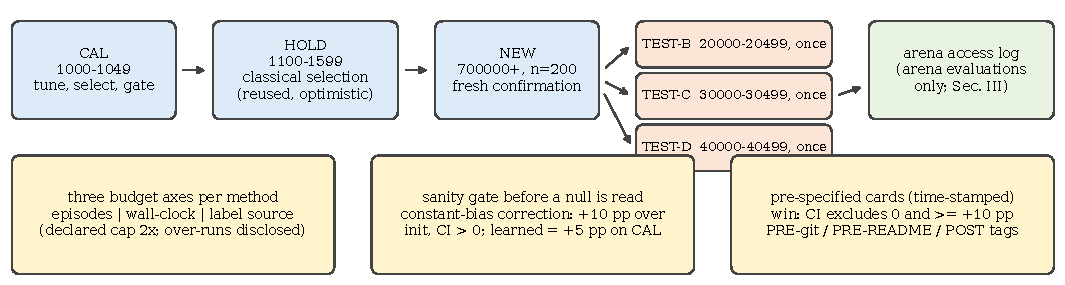
\includegraphics[width=\textwidth]{fig_protocol}
\caption{Protocol overview: seed-set roles (top) and the three rules that govern every comparison (bottom). The access log records arena evaluations on TEST seeds only.}
\label{fig:protocol}
\end{figure*}

\textbf{Extended classical tooling.} The classical side is not frozen at the textbook controller. It has a ladder of tuned variants (retuned gains, integral action, robust CMA-ES tuning, online system identification, and for whip an extended model class with 13 parameters; Section~\ref{sec:setup}). We call this tooling \emph{extended on the same footing} as the learner's, not equal on every axis: the classical side receives the generative parameter distribution as bounds and priors, and the learner receives it as simulated training data with labels.

\textbf{Three-axis budgets.} Every method reports episodes, wall-clock and label source, and the declared cap is 2$\times$ the classical episode budget. The learned side exceeded the cap in 4 of the 8 spikes of Appendix~\ref{app:budget}: it used 2.3$\times$ in the juggling PPO run, about 7$\times$ in the whip PPO sweep, 9--17$\times$ in the estimator duel and 3.2$\times$ in the idealised-whip re-run; in the other direction the classical tuning used about 7.7$\times$ the simulation steps of one RL policy in the first tracking study (Appendix~\ref{app:budget}). We report these ratios instead of equalising them.

\textbf{Pre-specified rules.} Hypotheses, metrics and decision rules are written in time-stamped, version-controlled cards (no external registry). A \emph{win} requires a paired bootstrap CI that excludes 0 and a gain of at least 10\% (tracking) or +10\pp\ (success rate); the +10\pp\ bar is our own choice and is not derived from a noise floor. Multiple tests inside one hypothesis family use Holm correction. Git order (rule committed before result) was verified for six early spikes (and for the headline rules of three more) and for the two locked-set runs of Section~\ref{sec:k3}; for ten spikes (01, 02, 03a, 04, 11a, 13b, 15b--15d, 16a) it cannot be shown because rule and result share a commit or the rule lived in a task prompt (Table~\ref{tab:audit}). No case was found in which git shows a rule committed after its result (Appendix~\ref{app:audit}). We therefore tag each result as pre-specified in git (\textbf{PRE-git}), pre-specified in a spike README only (\textbf{PRE-README}), or post hoc (\textbf{POST}). Because ``no win at +10\pp'' is not ``matched'', we add post hoc two one-sided tests (TOST) from the 90\% CI at $\pm10$ and $\pm5$\pp; only rows whose whole 90\% CI lies inside the margin are called equivalent. CIs and $p$-values are not corrected across spikes.

\textbf{Disjoint seed sets with roles.} Table~\ref{tab:seeds} lists the sets. Tuning and selection use CAL; HOLD selected the best classical baseline in two spikes and was then reused, so it is optimistic for the classical side; the locked sets TEST-B, TEST-C and TEST-D were each evaluated once.

\begin{table}[t]
\centering
\caption{Seed sets. ``Locked'' sets were used once for the evaluation named in the last column.}
\label{tab:seeds}
\small
\begin{tabular}{@{}p{0.9cm}p{2.6cm}rp{3.1cm}@{}}
\toprule
Set & Seeds & $n$ & Role \\ \midrule
CAL & 1000--1049; +2000--2149 in spikes 13a--15c & 50 (200) & tuning, selection \\
HOLD & 1100--1599 & 500 & classical selection; reused \\
TEST & 0--49 & 50 & older spikes; reused for juggling \\
TEST-B & 20000--20499 & 500 & locked, realistic whip (Sec.~\ref{sec:k2}) \\
TEST-C & 30000--30499 & 500 & locked, ladder (card v8) \\
TEST-D & 40000--40499 & 500 & locked, plan selection (card v9) \\
NEW & 700000+ & 200 & fresh confirmation \\
\bottomrule
\end{tabular}
\end{table}

\textbf{Sanity gate and learning check.} Before a learner's null is interpreted, the learner must learn a known-learnable correction: a constant torque bias injected after a probe, with a pass of +10\pp\ over its initialisation with a CI above 0. A learner counts as having \emph{learned} only if its CAL-selected checkpoint beats initialisation by at least 5\pp. The first gate passed marginally: with the exploration log-std $-1.5$ and 3M steps, PPO gained +10.2\pp\ [4.8, 15.6] on HOLD ($n{=}500$), best of 8 gate runs, 0.2\pp\ above the threshold, judged on $n{=}500$ instead of the pre-specified $n{=}200$; the zero-residual rule ($\le$40\%) was not met and SAC did not pass. The gate taught a lesson: the default exploration scale (log-std $-3.5$, 0.36\,Nm) gave $-3.0$\pp\ [$-8.5$, +2.5] and learned nothing, while $-2.0$ gave +7.8\pp\ [3.0, 12.8]. Later gates are single-seed shots (Appendix~\ref{app:budget}), so every RL null below reads ``not learned under this recipe'', never ``cannot learn''.

\textbf{Audit log.} Every arena evaluation on TEST seeds appends a line to a log, which has 111 lines. The log covers arena evaluations only: the TEST evaluations of the first five spikes ran outside it, so the line count is not the number of locked-set accesses and must not be quoted alone. The three locked sets of Table~\ref{tab:seeds} were each accessed once.

\section{Experimental Setup}
\label{sec:setup}


\textbf{Arm and simulator.} All experiments run in MuJoCo with planar serial arms. The default arm has two links (0.5 and 0.4\,m, 1.0 and 0.8\,kg); the whip uses a three-link arm (0.40, 0.35 and 0.25\,m; 1.0, 0.8 and 0.5\,kg; 0.2\,kg tip payload). A task, a robot, a controller and a list of perturbations plug into one environment interface. Controllers see only the nominal model; perturbations change the true plant (the list of perturbations is in Appendix~\ref{app:replication}). Control runs at 5\,ms.

\begin{table*}[t]
\centering
\caption{The eight settings cover three tasks, and each pairs learned methods with its own strongest classical baseline. ``Strongest classical'' is the comparator of Table~\ref{tab:cross}; on S7 it changed from R0 (the fitted-parameter classical pipeline, T-adapt3-full) to C-ens (the classical Laplace ensemble with robust plan selection) during the study (Section~\ref{sec:k3}). W0 (no plant weakness) and W3 (unmodelled friction) are conditions of the tracking task; L-est and L-dec4 are learned parameter estimators and B is the learned ensemble (Section~\ref{sec:setup}); T-robust, T-adapt and T-adapt3-full are classical controllers of increasing tooling. TEST, HOLD, TEST-B/C/D and NEW are the seed sets of Table~\ref{tab:seeds}.}
\label{tab:settings}
\small
\begin{tabular}{@{}lp{3.6cm}p{3.7cm}p{4.6cm}p{3.4cm}@{}}
\toprule
 & Task and condition & Strongest classical & Learned methods & Evidence sets \\ \midrule
S1 & tracking, no weakness (W0) or friction (W3), 2-link & C1: gains retuned by CMA-ES & residual PPO (5 seeds) & TEST \\
S2 & tracking + sensor noise + 30\,ms delay & C1-new (retuned for noise and delay) & residual PPO & TEST \\
S3 & tracking, clean nominal plant & CTC+LQR teacher (exact) & BC, MIP, flow-1, flow-10, DDIM-10 students & HOLD, fresh seeds \\
S4 & juggling, one known error (pilot) & one-parameter retuned mirror-law teacher & residual PPO & TEST \\
S5 & juggling, wide unknown error & T-robust (CMA-ES over the error distribution) & residual PPO, SAC, PPO with oracle observation & TEST, HOLD, fresh \\
S6 & whip, idealised (noise-free, in model class) & T-adapt (online identification) & L-est, residual PPO, PPO with oracle observation & TEST, HOLD, fresh \\
S7 & whip, realistic conditions & R0 (T-adapt3-full), later C-ens & L-est, L-dec4, ensembles (B), residual PPO, SAC & TEST-B/C/D, HOLD, NEW \\
S8 & whip, privileged-teacher distillation & T-adapt3-full & students on multimodal and canonical teacher data & NEW \\
\bottomrule
\end{tabular}
\end{table*}

\textbf{Seven tasks and where each is used.} The task set is figure tracking (a tool-tip glyph), pole balancing, Push-T, ball juggling, ball catching, ball tossing into a basket, and whip (Fig.~\ref{fig:tasks}). Learned-versus-classical comparisons with a full protocol cover tracking, juggling and whip (settings S1--S8, Table~\ref{tab:cross}). Pole balancing was run only on the classical ladder; catching, tossing and Push-T have classical pilots (5--20 demo seeds) and, in Appendix~\ref{app:breadth}, residual-PPO mini-comparisons that add breadth but not evidence for K2.

\textbf{Whip.} The arm flings a chain of ten capsules (0.10\,m, 0.015\,kg each, hinged at the tip) so that the \emph{chain tip} passes within 0.08\,m of a target 1.15--1.70\,m from the shoulder, outside the arm's 1.0\,m reach, within 2.5\,s. The chain state is not observed. ``Realistic conditions'' add encoder noise (1e-3\,rad, 1e-2\,rad/s), actuator noise $U(0.01, 0.02)$\,Nm, Coulomb friction $2\text{e-}3\,\text{Nm} \times U(0.5, 1.5)$ and per-link mass factors $\exp U(-0.3, 0.3)$. These magnitudes are our choice, set before the results, and are not derived from hardware. Success is the primary metric.

\textbf{Classical ladder.} For tracking the ladder runs proportional-integral-derivative control (PID), computed torque (CTC) with a linear-quadratic regulator (LQR), written CTC+LQR, iterative LQR (iLQR), iLQR in a model-predictive-control loop (iLQR-MPC) and model-predictive path-integral control (MPPI). For tuning, C0 is the untuned teacher, C1 retunes Kp/Kd or Q/R with the covariance-matrix-adaptation evolution strategy (CMA-ES) on the calibration seeds CAL, and C2 adds an integral term. For juggling and whip we use T-nom (nominal), T-robust (CMA-ES over the perturbation distribution), T-adapt (online system identification from a short probe) and, for realistic whip, T-adapt3 with an extended model class (length scale, ten chain-link masses, damping, Coulomb friction; 13 parameters). Its fitted-parameter pipeline is the baseline called R0 below. On whip the plan comes from CMA-ES keyframes tracked by computed torque.

\textbf{Learned methods.} Imitation students are a multilayer perceptron (MLP) trained by behaviour cloning (BC, with DART noise or DAgger where stated), MIP (two-step regression), flow matching with 1 or 10 steps, and a denoising-diffusion-implicit-model diffusion policy with ten steps (DDIM-10). Residual RL is PPO (SAC in sensitivity runs) on top of the strongest classical controller, with a residual capped at 12\,Nm in juggling and whip; the network and training recipe are in Appendix~\ref{app:budget}. Learned estimators map a short probe to the plant parameters: L-est is an MLP on the probe's tracking residuals (12{,}000 probe-only training episodes, simulator labels), and L-dec4 is a GRU on the raw probe time series with a decision-weighted loss and four times the data, with three training seeds. Ensembles average the estimated parameters of the three frozen L-dec4 networks. B is this learned ensemble used with robust plan selection (Section~\ref{sec:k3}), L-ens the same ensemble without it, and C-ens the classical counterpart of B: robust plan selection over parameter samples drawn from a Laplace (Gaussian) approximation around the classical fit. All training seeds are at least 500{,}000.

\textbf{Exploration scale.} The one residual-PPO parameter we found to matter most is the exploration log-std (Section~\ref{sec:protocol}); the rest of the recipe is in Appendix~\ref{app:budget}.

\textbf{Reproducibility.} Each result table is regenerated by a script from stored per-episode data, with the exception of runs that depend on untracked intermediate files; locked-set runs (TEST-B, TEST-C, TEST-D) were once-only and must not be repeated. All training seeds are at least 500{,}000 so that no training episode overlaps an evaluation set.

\textbf{Headroom ladder.} On whip we measure what each source of error costs with a fixed-order ladder on the same pipeline. R0 is the fitted-parameter pipeline; R1 gives it the true plant parameters; R2 adds the true chain state; R4 is an oracle planner with no probe time; R5 uses the canonical oracle. Paired differences between rungs give the size of each block. We also run the reverse order (true chain state first). R3, an oracle that starts from rest and waits 0.6\,s, was run on HOLD and NEW only (Appendix~\ref{app:replication}), not on the locked sets.

\textbf{Statistics.} Paired percentile bootstrap, 95\% CI, per comparison, with $10^4$ to $2{\times}10^4$ resamples depending on the script. ``Recovered fraction'' is $(\text{X}-\text{R0})/(\text{R1}-\text{R0})$ with the same resample in numerator and denominator. Holm correction applies within a hypothesis family: three hypotheses for the TEST-C card and four for the TEST-D card, both on one-sided bootstrap $p$-values at family $\alpha=0.05$.

\section{Results}
\label{sec:results}

\subsection{No learned method cleared the \texorpdfstring{+10\,pp}{+10 pp} bar against its strongest classical baseline}
\label{sec:k2}

No learned method cleared the bar in any setting. Out of 8 enumerated settings, none has a learned method with a CI above 0 and a gain of at least +10\pp\ (or 10\% RMSE) over the strongest classical baseline (Table~\ref{tab:cross} and Fig.~\ref{fig:forest} give the learned-minus-classical contrast per setting). The positive exceptions compare against weaker baselines: residual PPO against the untuned tracking teacher (+16.7\% RMSE), against the untuned juggling teacher (+292\% median hits; a one-parameter retune also reaches 100 hits), and against the weaker T-adapt of the juggling study (+9.3\pp\ [2.7, 17.3]).

\begin{table*}[t]
\centering
\caption{No learned method beats the strongest classical baseline by the +10\pp\ (or 10\% RMSE) bar in any setting; only the comparison with the weaker R0 does ($^\dagger$). Entries are learned minus strongest classical: success settings in percentage points, tracking in relative RMSE change (positive = learned better). Symbols: R0 is the fitted-parameter classical pipeline on whip (T-adapt3-full), which is no longer the strongest classical there; C-ens is the classical Laplace ensemble with robust plan selection; B is the learned ensemble with robust plan selection; L-est, L-est-full and L-dec4 are learned parameter estimators; T-robust, T-adapt and T-adapt3-full are classical controllers of increasing tooling, C1 and C1-new retuned classical gains; D-canon and D-multi are student training sets from the canonical and the multimodal teacher. S5, S6 PPO rows use the exploration scale chosen by the gate (single seed); the older rows with the default scale are in the source tables. TEST ($n{=}50$) was reused for juggling by three spikes; HOLD was reused (Section~\ref{sec:protocol}). Budget ratios per setting are in Appendix~\ref{app:budget}. The pilot S4 has no row here (see the equivalence summary in Appendix~\ref{app:audit}). This table is generated from result files by \texttt{figures/make\_figs.py}.}
\label{tab:cross}
\small
\begin{tabular}{@{}llrlrl@{}}\toprule
Set. & Learned vs.\ classical & $n$ & Seeds & $\Delta$ [95\% CI] & Learner \\ \midrule
S5 & PPO vs T-robust & 500 & HOLD & $-$23.8 [$-$26.9, $-$20.7] & degrades \\
S6 & PPO vs T-adapt & 500 & HOLD & $-$17.6 [$-$20.3, $-$14.9] & degrades \\
S6 & L-est vs T-adapt & 50 & TEST & $-$15.3 [$-$22.0, $-$8.7] & estimator \\
S7 & PPO vs R0 & 500 & HOLD & $-$2.1 [$-$5.2, +1.1] & not learned \\
S7 & L-est-full vs R0 & 500 & TEST-B & +0.9 [$-$3.5, +5.4] & estimator \\
S7 & L-dec4 vs R0 (H14) & 500 & TEST-C & +6.1 [+1.5, +10.7] & estimator \\
S7 & B vs C-ens (H16a) & 500 & TEST-D & +5.6 [+0.6, +10.6] & estimator + selection \\
S7 & B vs R0 (weaker baseline)$^\dagger$ & 500 & TEST-D & +16.2 [+11.0, +21.4] & estimator + selection \\
S8 & MIP D-canon vs T-adapt3-full & 200 & NEW & $-$12.0 [$-$19.8, $-$4.0] & BC student \\
\midrule
\multicolumn{6}{@{}l}{Tracking, relative RMSE change in \% (positive = learned better)} \\
S1 & PPO vs C1 (W0 clean) & 50 & TEST & $-$7.1 [$-$13.8, +0.3] & RL, 5 seeds \\
S2 & PPO vs C1-new (noise+delay, clean) & 50 & TEST & $-$21.7 [$-$25.7, $-$17.9] & RL, 5 seeds \\
S2 & PPO vs C1-new (noise+delay, disturbed) & 50 & TEST & $-$2.6 [$-$4.5, $-$0.7] & RL, 5 seeds \\
S3 & BC student vs teacher & 500 & HOLD & $-$0.8 [$-$1.0, $-$0.6] & imitation \\
S3 & flow-1 student vs teacher & 500 & HOLD & $-$0.5 [$-$0.7, $-$0.4] & imitation \\
S3 & DDIM-10 student vs teacher & 500 & HOLD & $-$6.2 [$-$6.7, $-$5.7] & imitation \\
\bottomrule\end{tabular}

\end{table*}

\begin{figure*}[t]
\centering
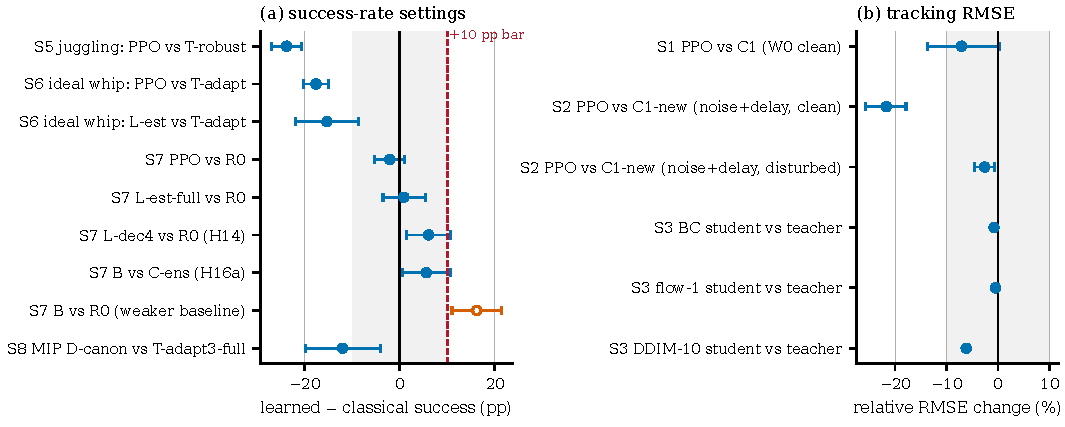
\includegraphics[width=\textwidth]{fig_forest}
\caption{No learned method clears the +10\pp\ bar against its strongest classical baseline; the single hollow point does, but only against the weaker baseline R0 (the fitted-parameter classical pipeline on whip). Learned minus classical across settings. Left: success-rate settings, grey band $\pm10$\pp, dashed line at the +10\pp\ bar. Right: tracking settings in relative RMSE. Bars are 95\% bootstrap CIs; the equivalence (TOST) calls in the text use 90\% CIs, for example [2.2, 9.9] for H14 (L-dec4 vs R0). Evidence sets differ across rows (Table~\ref{tab:cross}).}
\label{fig:forest}
\end{figure*}

Tracking (S1--S3) has little headroom by construction. With a retuned computed-torque controller there is no decisive difference from residual PPO on four clean and disturbed cells (S1: none of the four 90\% CIs decides at $\pm10\%$). With noise and a 30\,ms delay the retuned classical controller is better by 21.7\% clean and 2.6\% disturbed (S2). All five imitation students match the teacher on HOLD with fresh references, 0.5\% to 6.2\% worse in RMSE with CIs inside $\pm10\%$ (S3; the teacher is exact on the clean nominal plant).

In juggling and idealised whip (S5, S6), residual PPO degrades its base. With the gate-chosen exploration scale it loses 23.8\pp\ [20.7, 26.9] and 17.6\pp\ [14.9, 20.3] on HOLD, and 23.0\pp\ and 18.7\pp\ on fresh seeds. The idealised whip base is at 96.8\%, so a +5\pp\ learner effect is impossible there, and for S5 the gate is easy, so it tests plumbing rather than sensitivity.

In realistic whip (S7), neither learned estimators (+0.9\pp\ [$-3.5$, 5.4] on TEST-B) nor PPO ($-2.1$\pp\ [$-5.2$, +1.1]) beat the strongest classical baseline at that time. Eleven PPO and 2 SAC configurations and a 12M-step run all stayed within $-3$ to +2\pp\ of initialisation. Privileged-teacher distillation (S8) leaves all students 12--45\pp\ below T-adapt3-full.

Three of the 8 settings (S5, S6, S7 PPO) had a learner that did not learn, so they cannot show that classical is better. The post hoc TOST rows show equivalence at $\pm10$\pp\ only for some rows (for example S3, S7 estimators and S7 PPO) and clearly worse learners for others; S1 is undecidable and no row has the learner clearly better by more than 10\pp\ (Appendix~\ref{app:audit}). Where we write ``no detectable difference at the +10\pp\ bar'' we do not claim equivalence.

Realistic whip is the setting where headroom is largest, so its history is worth stating in one place. On the locked TEST-B set ($n{=}500$, one evaluation) R0 (T-adapt3-full), the strongest classical baseline at that time, scored 65.6\% [61.4, 69.8], the oracle 89.2\%, and the total headroom was +23.6\pp\ [18.8, 28.4]. The learned estimator with per-link labels (L-est-full) differed from R0 by +0.9\pp\ [$-3.5$, 5.4], and a version without per-link mass labels by $-1.2$\pp\ [$-5.8$, 3.5]; the pre-specified hypothesis that a learned estimator beats R0 by 10\pp\ was not supported. Residual PPO on that set was 0.0\pp\ [$-4.0$, 4.0], but it used the default exploration scale shown by the gate to be unlearnable, so we use the later 3-seed run ($-2.1$\pp) instead. These sets motivated the ladder of Section~\ref{sec:k3}.

Whip is the exception that carries the qualification of K2. Against R0 alone, the learned ensemble B clears the bar on the locked TEST-D set: B$-$R0 is +16.2\pp\ [11.0, 21.4]. But a classical Laplace ensemble, C-ens, also beats R0 by +10.6\pp\ [5.8, 15.4], and against C-ens the learned side is ahead by +5.6\pp\ [0.6, 10.6] (Section~\ref{sec:k3}). C-ens exists because an earlier, unlocked study had shown B ahead of R0; the hypothesis card v9 was written after C-ens was frozen and before TEST-D. A learned advantage of 10\pp\ or more therefore cannot be excluded, and we do not write ``no learned method wins by 10\pp'' without this qualification.

\subsection{On realistic whip, parameters are the largest rung and robust plan selection recovers a large share of that gap}
\label{sec:k3}

On the locked set TEST-C, the true-parameter step is the largest single rung of the headroom ladder. Fig.~\ref{fig:ladder} shows the ladder ($n{=}500$, card v8 committed before the run). The fitted-parameter pipeline R0 reaches 65.6\% [61.4, 69.6]; true parameters (R1) reach 83.2\% [79.8, 86.4]; adding the true chain state (R2) gives 88.6\%; the oracle R4 reaches 93.0\% [90.6, 95.2]. The parameter step R1$-$R0 is +17.6\pp\ [12.6, 22.6] (hypothesis H13 supported, Holm $p=0.00015$). The probe cost R4$-$R2 is +4.4\pp\ [0.8, 7.8]: small but not zero, and the pre-specified bound (upper end below +5\pp) failed (H13b not supported). The chain-state step is R2$-$R1 +5.4\pp\ [1.6, 9.4], and the total headroom R4$-$R0 is +27.4\pp\ [22.6, 32.2]. In the reverse order the chain state first adds +4.8\pp\ [$-0.8$, 10.6] and the parameters then add +18.2\pp\ [13.4, 23.0], so the parameter step is about +18\pp\ in both orders. The same step appeared on the reused HOLD (+16.8\pp\ [12.0, 21.6]) and fresh NEW seeds (+13.0\pp\ [4.5, 21.5]; Appendix~\ref{app:replication}). Parameter estimation is therefore the \emph{largest single rung} of this ladder, not \emph{the} cause: rung sizes depend on order and are not additive.

\begin{figure}[t]
\centering
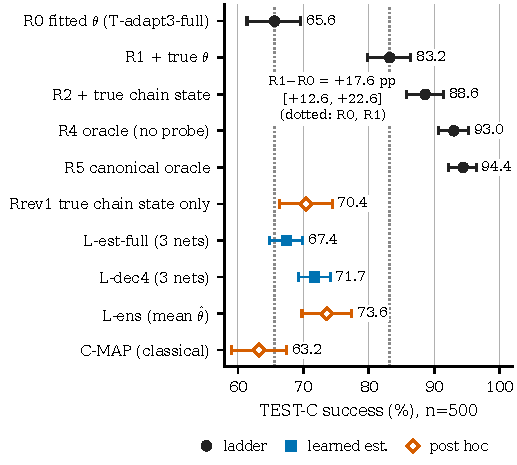
\includegraphics[width=\columnwidth]{fig_ladder}
\caption{Parameter estimation is the largest single rung of the headroom ladder on realistic whip (locked TEST-C), and learned estimators recover only part of it. Rungs: R0 fitted parameters, R1 true parameters, R2 adds the true chain state, R4 oracle planner with no probe time, R5 canonical oracle, Rrev1 true chain state only. Orange open markers are post hoc, descriptive rows. Dotted lines mark R0 and R1. Learned estimators sit between R0 and R1; the classical maximum-a-posteriori (MAP) fit with multi-start sits below R0.}
\label{fig:ladder}
\end{figure}

A learned estimator recovers only part of the parameter gap on TEST-C. The pre-specified estimator duel (H14) compares L-dec4 with R0. L-dec4$-$R0 is +6.1\pp\ with a 90\% CI of [2.2, 9.9], inside $\pm10$\pp, but the Holm-adjusted $p$ is 0.094, so equivalence is \emph{not confirmed} after Holm (the unadjusted TOST passes by 0.1\pp). The estimator recovers 0.34 [0.10, 0.53] of the R0-to-R1 gap, L-est-full 0.10 [$-0.18$, 0.31], and a classical MAP fit with multi-start $-0.14$ [$-0.56$, 0.16] (descriptive). On the reused HOLD the same duel had given +1.1\pp\ [$-3.3$, 5.7], a 4--7\% recovered fraction with a CI that crosses 0; the locked number supersedes it. Parameter error falls a lot (log-damping RMS 0.693 to 0.323) while success moves far less, so precision rather than direction of the error is the issue. Success is also noisy in $\hat\theta$: re-running identical models with float-rounding changes moved HOLD success by up to 3.6\pp.

Robust plan selection recovers a large share of the parameter gap on the locked set TEST-D, for either side. Both selection rules score 8 plus 3 candidate swings (whip plans) in four plausible plants and choose by a worst-case or hit-fraction aggregate. B uses three frozen learned estimators; C-ens uses a Laplace posterior around the classical fit, the same rule on the classical side.

Fig.~\ref{fig:testd} shows TEST-D ($n{=}500$, card v9 committed before the run). R0 reaches 66.4\% [62.2, 70.6], R1 84.4\% [81.2, 87.6] (an R1$-$R0 gap of +18.0\pp), C-ens 77.0\% [73.2, 80.6] and B 82.6\% [79.2, 85.8]. The card's hypothesis H15, that C-ens beats R0, holds: C-ens$-$R0 is +10.6\pp\ [5.8, 15.4]. H15b, that B beats R0, holds: B$-$R0 is +16.2\pp\ [11.0, 21.4]. The share of the R1$-$R0 gap recovered is 0.59 [0.36, 0.82] for C-ens and 0.90 [0.68, 1.16] for B. H16a, that B beats C-ens, holds under Holm: B$-$C-ens is +5.6\pp\ [0.6, 10.6] (Holm $p=0.032$). H16b, that the B advantage is below 10\pp, is \emph{not supported}: the card's rule requires the 95\% CI upper end below +10\pp, and it is 10.6. The card is internally inconsistent here: the rule uses the two-sided 95\% CI, while the Holm step uses a one-sided $p$ that corresponds to the 90\% CI (upper end 9.8, $p=0.043$). We apply the rule text, so a learned advantage of 10\pp\ or more is not excluded.

\begin{figure}[t]
\centering
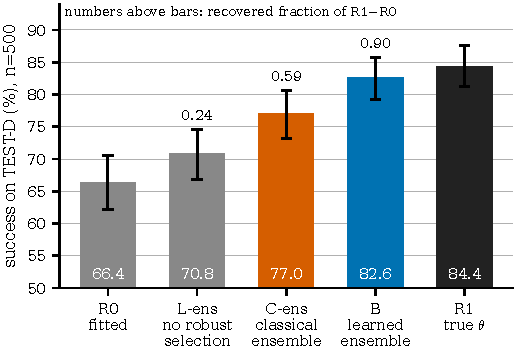
\includegraphics[width=\columnwidth]{fig_testd}
\caption{Robust plan selection recovers a large share of the parameter gap on the locked set TEST-D: 0.59 of the R1$-$R0 gap with the classical ensemble C-ens and 0.90 with the learned ensemble B, which leads C-ens by +5.6\pp. Bars: success with 95\% CI; numbers above the bars: recovered fraction of the R1$-$R0 gap. R0 uses fitted parameters and R1 the true parameters. C-ens is the classical Laplace ensemble with robust plan selection, B the learned ensemble with robust plan selection, and L-ens the same frozen learned estimators as B without robust selection. The y axis starts at 50\%.}
\label{fig:testd}
\end{figure}

A control shows that the gap lies in choosing among candidates rather than in the candidate pool: the best of the executed candidates would have succeeded in 99.8\% of episodes for both runs. The reproduction checks, the agreement of the base candidate with R0 and the winner's-curse effect in the selection of B and C-ens are in Appendix~\ref{app:replication}.

Without robust selection the learned estimators add little on TEST-D. The learned estimator without robust selection gives only +4.4\pp\ [$-1.4$, 10.0] on TEST-D (L-ens, recovered 0.24); on TEST-C the same ensemble gave +8.0\pp\ [2.6, 13.6] (descriptive). The two locked sets differ by several points for the same frozen networks, which fits the noise floor above. Costs differ in the other direction: the classical ensemble needs about 63.3\,s of CPU per episode against 20.4\,s for B, and the learned side paid 13{,}120 training episode-equivalents with simulator labels. Post hoc and descriptive results, not in any verdict, are a 9-network learned ensemble (84.4\% on TEST-D, recovered 1.00 [0.77, 1.29]), the reverse-order ladder, L-ens and C-MAP.

The classical ensemble C-ens recovers 0.59 [0.36, 0.82] of the R1$-$R0 gap without better parameters, and we read this as robust plan selection mattering more than a better point estimate. That reading is an interpretation of the 0.59 fraction, not a test:  averaging the model score over four nearby plants may simply reduce variance in a success rate that is close to chaotic in $\hat\theta$, and we did not test this alternative.

\subsection{A multimodal teacher: canonicalising it helps more than a richer student}
\label{sec:k4}

Canonicalising the teacher helps students more than a richer student does. When the whip teacher is the standard multimodal CMA-ES planner, re-planning the same situation varies by 0.96\,rad RMS, as much as plans for different situations (0.92\,rad); a continuation-warm-started canonical teacher varies by 0.27\,rad within a scenario against 0.73\,rad between scenarios. Replacing the multimodal teacher by the canonical one raised every student's success by 17.5--33.5\pp\ on NEW seeds (BC only, one data size, $n{=}200$; Fig.~\ref{fig:k4} in Appendix~\ref{app:k4}). The best generative student exceeded the MLP by +5.0\pp\ [$-0.3$, 10.2] on the multimodal teacher's data: below the +10\pp\ bar, not an equivalence result, and the best student was identified post hoc. Neither result has locked-set confirmation, and the canonical teacher also changes plan smoothness, so the gain combines multimodality removal with plan regularity.

\section{Discussion}
\label{sec:discussion}

Our data suggest three conditions for learning to add value over a strong classical controller, and only two of them were met. Under this protocol and in these settings, the conditions are, in order, as follows. First, headroom the classical toolbox cannot reach: it exists only on realistic whip (an oracle gap of +27.4\pp\ on TEST-C), while tracking ties and no juggling cell gained 10\pp\ from classical re-tuning in a small diagnostic. Second, a learner that passes the sanity gate on that gap at the control level: PPO and SAC did not on whip or juggling, and with the gate-chosen exploration scale PPO degraded S5 and S6 by 23.8 and 17.6\pp. Third, a planning step that does not trust one estimate. Robust plan selection, which scores candidates across several plausible plants, recovers 0.59 [0.36, 0.82] of the parameter gap with a classical Laplace ensemble and 0.90 [0.68, 1.16] with learned estimators, with the learned side ahead by +5.6\pp\ [0.6, 10.6]. The first and third conditions were met in our data; the second was not. Our reading is an inference rather than a test (Section~\ref{sec:k3}). We read the result as follows: the ingredient that helped was robust plan selection, a \emph{decision rule over a set of plausible plants} that either side can use, plus an advantage for learned estimators trained with simulator labels (+5.6\pp\ [0.6, 10.6]) that may reach 10\pp\ or more. We did not find a control-level learner (PPO, SAC, imitation student) that beats the strongest classical controller, and we have not shown that control-level learning is unattainable.

One piece of counter-evidence argues against reading K2 as ``classical is at least as good''. Under actuator noise four times larger, the classical T-adapt3-full lost 12.5\pp\ while the learned estimator did not: the paired difference is $-16.5$\pp\ [$-28.5$, $-5.0$] on HOLD ($n{=}200$, frozen methods, no re-tuning at the higher noise; Appendix~\ref{app:replication}). This is weak evidence, but together with the locked-set advantage of H16a it argues against a blanket reading of K2.

Three features could make the headline contrast of robust plan selection look cleaner than it is. The classical ensemble uses the generative parameter distribution as a prior, so it is not neutral; the learned estimators see the same distribution as training data. Both selection rules were picked on CAL among 20 or 22 variants, and the multi-start classical family, an obvious alternative, was degenerate in our implementation (it found no distinct second solution in 439 of 500 HOLD episodes). Finally, the success rate is close to chaotic in the estimated parameters, so differences of a few points between pipelines sit within the replicate noise we measured. The locked TEST-D set controls the selection effect but not the other two.

The null does not say that learning is worse. Three of eight settings had a learner that did not learn; the RL recipe was one family; 5 of the 8 settings have little or no headroom; and the +10\pp\ bar is ours. The comparison is also not equal on every axis: the learned estimators used 9--17$\times$ the classical episodes and simulator labels, whereas the classical ensemble costs about three times the CPU time per episode at test time.

For benchmark design, our results suggest four practices. Report the sanity gate and an oracle with every learned-versus-classical table, because a null from a learner that cannot learn a trivial correction is uninformative. Tag each result as pre-specified or post hoc; log locked-set accesses; and state which classical baseline is meant when the baseline changes during the study. Our own change of the strongest classical baseline on whip (R0 to C-ens) moved the learned advantage from +16.2\pp\ to +5.6\pp.

\section{Limitations}
\label{sec:limitations}

\begin{enumerate}
\item \textbf{RL did not learn where it matters.} On realistic whip, 13 tuned PPO and SAC configurations and a 12M-step run stayed within $-3$ to +2\pp\ of initialisation; the first gate passed marginally and later gates are single-seed. Our null is ``not learned under this recipe'', not ``cannot learn''.
\item \textbf{Holdout reuse.} HOLD selected the best classical baseline and was then reused, so classical numbers are optimistic there (R0 69.2\% on HOLD against 65.6--66.4\% on the three locked sets).
\item \textbf{Our own realism.} Noise, friction and mass magnitudes were set by us, not derived from hardware.
\item \textbf{One simulator, one dominant task.} All results are MuJoCo and the mechanistic claims (K3, K4) rest on whip alone; there is no second engine or hardware.
\item \textbf{Budgets, multiplicity and the order of the classical upgrade.} Budget ratios were unequal (up to 9--17$\times$); Holm applies within a hypothesis only; the classical ensemble was added after the learned result was seen, and the learned advantage +5.6\pp\ [0.6, 10.6] does not exclude 10\pp.
\item \textbf{Numerical warnings.} The TEST-D log contains 125{,}555 MuJoCo ``simulation unstable'' warnings; a re-run on 100 holdout episodes attributes 92--98\% of them to planner model rollouts and none to the executed plant (0 of 100 executed episodes diverged), but the check is $n{=}100$ on holdout only.
\end{enumerate}
Appendix~\ref{app:audit} gives the full text of these items and the forking paths.

\section{Conclusion}
\label{sec:conclusion}

Under a fair, pre-specified and budget-disclosed protocol, with extended classical tooling, no learned method beat the strongest classical baseline by +10\pp\ in 8 tracking, juggling and whip settings. Only realistic whip has headroom. There, the largest rung of the headroom ladder is parameter estimation (+17.6\pp\ on TEST-C). On the second locked set, TEST-D (gap +18.0\pp), robust plan selection, a decision rule that scores candidate swings under several plausible plants and that either side can use, recovers a large share of the gap: 0.59 for the classical side alone and 0.90 for the learned side, and the learned side keeps a lead of +5.6\pp\ [0.6, 10.6] with a 10\pp\ advantage not excluded.

On a multimodal whip teacher, replacing it by a canonical one raised every student's success by 17.5--33.5\pp, more than the best generative student added over an MLP (+5.0\pp\ [$-0.3$, 10.2]); this result has no locked-set confirmation. The protocol is reusable. Any other group can apply its sanity gate, its seed-set roles, its pre-specified cards and its access log to check whether a reported learned advantage survives an equally tuned classical baseline, though we have applied it only here. The evidence is one simulator and mostly one task. The next experiments we consider most informative are a control-level learner that demonstrably closes part of the oracle gap, a second task with headroom in a second simulator, and equal-effort classical tuning for the estimator duel.


\section*{Acknowledgment}
\emph{Use of AI tools.} The research question, the choice of tasks, every direction change and every decision recorded in the hypothesis cards were made by the author. Most of the code, the execution of the experiments, the statistical analysis and the drafting of this text were carried out by AI agents (Anthropic's Claude models, used through Claude Code) working under the author's direction; internal reviews of the drafts were also simulated with AI agents. The author checked the results reported here and takes full responsibility for the content.

\bibliographystyle{IEEEtran}
\bibliography{refs}

\clearpage
\onecolumn
\appendices
\small

\section{Deviations and Audit}
\label{app:audit}

\subsection{Pre-specification audit}
Table~\ref{tab:audit} gives, for each spike, whether git shows the rule committed before the result. Timestamps are local commit times on one author clock; the repository has no external timestamping. ``YES'' means the rule text is in a commit strictly earlier than the first commit containing the result; ``UNPROVABLE'' means both arrive in one commit or the rule lived in a task prompt. No case was found in which git shows a rule committed after its result.

\begin{table}[htbp]
\centering
\caption{Git order of rule and result.}
\label{tab:audit}
\begin{tabular}{@{}p{3.3cm}p{9.2cm}l@{}}
\toprule
Spike & Rule and note & Order \\ \midrule
01, 02, 03a & Cards v1/v2, same snapshot commit as results; W1/W2 strengths set after a teacher-only look at TEST (spike02) & UNPROVABLE \\
03b, 05, 06, 07, 09b, 10b & Cards v2--v7.1 committed 1--4 h before results. Deviations: PPO recipe pre-lesson (03b); retroactive log entry (05); checkpoint selection added after round 1 (06); PPO not fixed before TEST (07); plant step changed after CAL tuning and dose curve run after locked TEST-B (10b) & YES \\
04 & H7 written in the result commit and amended after seeing the delay break the old C1 & UNPROVABLE, amended \\
11a, 13b & Rule in a task prompt or README of the result commit & UNPROVABLE \\
12a, 13a, 14a & Headline rule in the decision log earlier; details in the result commit. 13a: gate bias fell back to 6\,Nm and the gate was judged on $n{=}500$ instead of 200 & YES for headline \\
15a (TEST-C) & Cards v8 and v8.1 committed on their own about 2 h before the run; v8.1 re-trained L-dec4, predictions identical to the stored ones & YES \\
15b, 15c, 15d & Rules in README section 0 only; X1 (15b) and the 9-network extension (15c) added after results and labelled post hoc & UNPROVABLE \\
15e (TEST-D) & Card v9 committed on its own 1 h 22 min before the run; the code was uncommitted at run time, and the gated step was finished by the orchestrator with unchanged code & YES (card) \\
16a & Rule in README section 0, same commit as results; code uncommitted at run start & UNPROVABLE \\
learn\_demo & Not pre-specified; hyper-parameters chosen after one TEST look; stale, superseded by S3 re-run & NO \\
\bottomrule
\end{tabular}
\end{table}

\subsection{The v9 card is internally inconsistent for H16b}
The card's H16b rule is ``$B-\text{C-ens}$, 95\% CI upper end below +10\pp''. Its Holm step uses a one-sided bootstrap $p$ for $H_0$: difference $\ge 10$, which corresponds to the 90\% CI. On TEST-D the 95\% upper end is 10.6 (rule fails), the 90\% CI is [1.4, 9.8], and the one-sided $p$ is 0.0432, which would pass at $\alpha=0.05$ alone. We treat the rule text as binding, so H16b is not supported, and never write that the advantage is below 10\pp. The card's pre-written sentence for this outcome, applied on Holm-surviving verdicts, reads that the learned advantage may be $\ge10$\pp\ and that the paper rewrites K2 accordingly; Section~\ref{sec:k2} does so.

\subsection{Order of the classical upgrade (C-ens)}
The classical ensemble C-ens was built \emph{after} the learned ensemble B had beaten R0 on holdout (a first commit at 18:07 on the day of the study) and was frozen in a second commit at 20:31; its selection was written to a file before holdout and new-seed collection, and the v9 card was written at 20:32, after C-ens was frozen and before TEST-D. B$-$C-ens is therefore a pre-specified locked contrast, but the classical comparator was built with the learned result in view. The rule was developed first for the learned side and then given to the classical side. C-ens was chosen on CAL among 20 ensemble variants (B among 22) and uses the generative parameter distribution as a prior (a disclosed, non-neutral choice); no Laplace-width sensitivity run was made, and the multi-start classical family was degenerate (439 of 500 holdout episodes without a distinct second solution). On the pre-locked sets the contrast was B$-$C-ens +7.0\pp\ [2.6, 11.4] (holdout) and +4.0\pp\ [$-3.0$, 11.0] (new seeds), verdict UNCERTAIN by the README rule.

\subsection{Audit log scope}
The log has 111 lines: 47 from the demo-student script, 56 from one MJX evaluation, one each for juggling spikes 05, 06, 07 (05 and 06 retroactively), whip spike 09b, TEST-C and TEST-D, and two for spike 10b (TEST-B and TEST). The log is written only by the arena's \texttt{evaluate}. The TEST evaluations of spikes 01, 02, 03a, 03b and 04 ran outside it; spikes 15b--15d and 16a added no lines because guards block the locked sets. TEST (seeds 0--49) was reused across several spikes, on the same task for juggling (05, 06, 07).

\subsection{Equivalence summary (post hoc TOST)}
Equivalent within $\pm10$ (whole 90\% CI inside): S2 disturbed, S3 (all five students), S4 restitution (pilot), S5 oracle-PPO (legacy), S7 L-est-full, L-est-eff, PPO (13a) and OOD. Within $\pm5$ as well: S2 disturbed, S3 BC, MIP and flow, S5 oracle-PPO, S7 L-est-full and PPO. Not decidable: S1 (all four cells), S6 oracle-PPO (legacy), S8 best D-canon student. Learned clearly worse (90\% CI below $-10$): S2 clean, S4 mass and sensing (pilot), S5 PPO ($-23.8$) and SAC, S6 PPO ($-17.6$) and L-est, S8 D-multi students. Learned clearly better beyond $\pm10$: none.

\subsection{Full limitations}
\begin{enumerate}
\item \textbf{RL did not learn in the settings that matter most.} On realistic whip, 11 PPO and 2 SAC configurations tuned on CAL, three seeds of 3M steps and a 12M-step run all stayed within $-3$ to +2\pp\ of initialisation; in idealised whip all six PPO runs were flagged not learned; in juggling the residual stayed at 0.15--0.18\,Nm of a 12\,Nm cap and 4 of 6 runs chose the first checkpoint. The gate passed marginally, only after raising the exploration scale, among 8 gate runs. The S5 and S6 re-runs degrade the base by 23.8 and 17.6\pp, but each gate is a single-seed shot, the S5 gate is easy, the S6 budget is 3.2$\times$ classical, the recipe was not swept on the real condition, and the asymmetric-critic gate failed. The null is ``not learned under about 3--12M steps, one recipe per setting and about 13 tuned configurations on whip''.
\item \textbf{Holdout reuse.} HOLD was used to choose best-classical in spikes 09b and 10b (on 300 of the 500 seeds) and then as the main evaluation set in spikes 13a, 13b and 14a. R0 is 69.2\% on HOLD against 65.6, 65.6 and 66.4\% on TEST-B, TEST-C and TEST-D. The multimodal-teacher result, the group split, the fragility sweep and the 9-network extension have no locked-set confirmation.
\item \textbf{Realistic conditions are our own choice.} The friction value is an estimate.
\item \textbf{One simulator.} No second engine, no hardware.
\item \textbf{Concentration on whip.} Five of the eight settings are tracking or juggling, where headroom is small or absent.
\item \textbf{Unequal tuning knobs.} The classical side tuned 5--13 parameters with 750--9{,}050 episodes and received the generative distribution as bounds and priors; the learned side used $10^4$--$10^5$ episodes and simulator labels. In the estimator duel the classical side tried only three strengthened variants.
\item \textbf{Forking paths.} W1/W2 strengths set after seeing TEST (spike02); hyper-parameters chosen after one TEST look (learn\_demo); RL recipe repaired after round 1 (spike06); PPO not fixed before TEST (spike07); plant step changed after CAL tuning and dose curve after the locked TEST-B (spike10b); post hoc analyses in spikes 13b and 14a. There is no correction across spikes, so positive exceptions are exploratory.
\item \textbf{Pipeline noise.} Re-running identical estimator models with float-rounding changes moved holdout success by up to 3.6\pp\ per model, comparable to several reported differences.
\item \textbf{Power and equivalence.} Most pre-specified tests had CI half-widths of 4--9\pp\ (TEST $n{=}50$ comparisons up to about 15\pp). ``No side wins at the 10\pp\ bar'' is not an equivalence test. Differences of +1 to +5\pp\ (for example the three-model ensemble, +4.8\pp\ [$-0.8$, 10.4]) cannot be excluded.
\item \textbf{Fairness of the plan-selection duel.} See the C-ens paragraph above; the learned side used 13{,}120 training episodes with simulator labels, and both sides are frozen by the v9 card.
\item \textbf{Pre-specified versus post hoc.} Besides the earlier spikes marked YES in Table~\ref{tab:audit}, only cards v8, v8.1 and v9 were committed on their own before their runs; spike15b/15c/15d rules are README-only; the 9-network extension, B9, the reverse-order ladder, S6-X1 and L-ens/C-MAP are post hoc or descriptive.
\item \textbf{Numerical warnings.} The check of the 125{,}555 warnings (4{,}621 on holdout) was a re-run on 100 holdout episodes; the full holdout and TEST-D check was not repeated. No executed episode record contained a non-finite outcome.
\item \textbf{Order of the classical upgrade.} See above.
\end{enumerate}

\section{Budgets and the RL Gate}
\label{app:budget}

\begin{table}[htbp]
\centering
\caption{Budget by spike (episodes, steps, wall-clock where reported). Counting conventions differ between steps, episodes and probe-equivalents; the spike09b classical design cost (about 1{,}300 episodes) is an estimate.}
\label{tab:budget}
\begin{tabular}{@{}p{2.2cm}p{7.3cm}p{3.7cm}@{}}
\toprule
Spike & Classical side / learned side & Ratio \\ \midrule
03a (tracking) & classical tuning 6.4M--9.0M steps; RL 2M steps per policy & classical about 7.7$\times$ (C1+C2, one weakness) \\
06 (juggling) & classical 118.2M steps; RL 121.0M & 1.02$\times$ \\
07 (juggling) & PPO and oracle about 144M steps (107.6M without out-of-memory reruns); SAC 27M & 2.3$\times$ (1.7$\times$) \\
10b (whip) & classical 11{,}300 episodes (2$\times$ cap 22{,}600); learned methods each inside the cap & within cap \\
13a (whip RL) & about 160k episodes vs 22.6k classical & about 7$\times$ \\
14a (estimator duel) & learned about 13{,}120 episode-equivalents vs classical about 1{,}500 & 9--17$\times$ \\
15b (S6 re-run) & 33k episodes vs 10{,}350 classical & 3.2$\times$ \\
16a (catch / toss / Push-T) & classical tuning 16{,}200 / 10{,}200 / 2{,}100 episodes; PPO 16{,}227 / 10{,}222 / 2{,}114 & about 1$\times$ \\
\bottomrule
\end{tabular}
\end{table}

\begin{table}[htbp]
\centering
\caption{All RL gates and checkpoint decisions (single seed or best-of-$N$ flagged). Differences are paired learned minus initialisation (gates) or minus base (real conditions), in pp.}
\label{tab:gates}
\begin{tabular}{@{}p{4.4cm}p{5.3cm}p{3.5cm}@{}}
\toprule
Gate or run & What is single-seed or best-of & Result \\ \midrule
13a gate, log-std $-3.5$ (default) & gate set $n{=}200$ & $-3.0$ [$-8.5$, +2.5] \\
13a gate, log-std $-2.0$ & HOLD $n{=}500$ & +7.8 [3.0, 12.8] \\
13a gate, log-std $-1.5$, 3M steps & best of 8 runs, CAL-selected & +10.2 [4.8, 15.6] \\
13a gate, SAC & single seed & +1.8 [$-3.4$, 7.0] \\
13a real condition & 11 PPO + 2 SAC configs, one seed each; confirmation 3 seeds & HOLD $-2.1$ [$-5.2$, 1.1]; NEW $-1.3$ [$-6.5$, 3.8]; 12M steps $-0.6$ [$-4.6$, 3.4] \\
15b S6 gate (bias 6\,Nm) & one seed, one shot & +15.4 [10.2, 20.6] \\
15b S5 gate (bias 1\,Nm) & one seed, one shot; easy gate & +63.2 [58.8, 67.4] \\
15b S6-X1 (weak base, post hoc) & CAL picks looked like +5.0, +11.5, +5.0 and vanished on disjoint seeds & holdout $-5.0$ [$-8.7$, $-1.5$]; fresh $-3.3$ [$-8.7$, +2.0] \\
15c asymmetric critic & two seeds, one extra attempt allowed; failed & +7.2 [2.0, 12.4]; +1.2 [$-4.0$, 6.4] \\
\bottomrule
\end{tabular}
\end{table}

\section{Replication on Reused and Fresh Seeds, and Sensitivity}
\label{app:replication}

\begin{table}[htbp]
\centering
\caption{Headroom ladder on HOLD ($n{=}500$) and NEW ($n{=}200$): success \% [95\% CI].}
\label{tab:replication}
\begin{tabular}{@{}lll@{}}
\toprule
Rung & HOLD & NEW \\ \midrule
R0 fitted & 69.2 [65.2, 73.2] & 69.0 [62.5, 75.5] \\
R1 true $\theta$ & 86.0 [83.0, 89.0] & 82.0 [76.5, 87.0] \\
R2 + chain state & 89.0 [86.2, 91.6] & 89.5 [85.0, 93.5] \\
R3 oracle at rest, waits 0.6\,s & 88.2 [85.4, 91.0] & 85.5 [80.5, 90.5] \\
R4 oracle & 90.8 [88.2, 93.2] & 87.5 [82.5, 92.0] \\
R5 canonical oracle & 92.0 [89.6, 94.2] & 92.5 [88.5, 96.0] \\
L-est-full (3 nets) & 64.7 [62.1, 67.3] & 66.7 [62.5, 70.8] \\
R1$-$R0 & +16.8 [12.0, 21.6] & +13.0 [4.5, 21.5] \\
R2$-$R1 & +3.0 [$-1.0$, 7.0] & +7.5 [1.0, 14.0] \\
R4$-$R2 & +1.8 [$-1.6$, 5.4] & $-2.0$ [$-8.0$, 4.0] \\
\bottomrule
\end{tabular}
\end{table}

On TEST-B the total headroom (T-oracle minus the best classical) is +23.6\pp\ [18.8, 28.4]. The R2$-$R1 step is significant on NEW but not on HOLD, and the R4$-$R2 sign flips, so these blocks are not replicated as real; the earlier suggestion that the oracle gap was mostly probe time and chain state was a winner's-curse artefact and is superseded. A post hoc group split on HOLD (wrong damping 18.4\pp, per-link masses 16.2, length 7.4, friction 4.6 when only that group is wrong) is non-additive and not used for claims.

\begin{table}[htbp]
\centering
\caption{Actuator-noise sweep, HOLD seeds 1100--1299 ($n{=}200$), paired drop relative to the $\times$1 noise level (pp [95\% CI]). Methods frozen, not re-tuned per level.}
\label{tab:fragility}
\begin{tabular}{@{}lrrr@{}}
\toprule
Method & $\times$2 & $\times$4 & $\times$8 \\ \midrule
T-adapt3-full & +0.5 [$-7.5$, 8.5] & $-12.5$ [$-21.5$, $-3.5$] & $-14.5$ [$-24.0$, $-5.0$] \\
L-est-full & +7.0 [$-1.5$, 15.5] & +4.0 [$-5.0$, 13.0] & $-0.5$ [$-10.0$, 9.0] \\
T-oracle & +0.5 [$-3.0$, 4.0] & $-3.5$ [$-7.0$, 0.0] & $-1.0$ [$-4.0$, 1.5] \\
\bottomrule
\end{tabular}
\end{table}

Under sensor noise the ordering is not distinguishable (T-adapt3-full $-10.0$\pp\ [$-19.5$, $-1.0$] at $\times$2, L-est-full +0.5 [$-8.5$, 9.5]). The paired difference of the two drops at actuator noise $\times$4 is $-16.5$\pp\ [$-28.5$, $-5.0$].

\textbf{Dose curve and out-of-distribution.} On HOLD ($n{=}200$ per level; run after the locked TEST-B), success of best classical / L-est-full / L-est-eff / T-oracle is 71.0 / 64.3 / 67.5 / 92.0 at $\times$0.5, 69.5 / 61.2 / 61.2 / 89.5 at $\times$1 and 53.0 / 60.3 / 56.8 / 91.0 at $\times$2. The paired L-est-full minus classical is $-6.7$ [$-13.5$, 0.2], $-8.3$ [$-16.2$, $-0.3$] and +7.3 [$-0.0$, 14.7]: a single point at the strongest condition. For estimators trained or tuned at $\times$0.5 and $\times$2 and evaluated at $\times$1, L-est-OOD minus T-adapt3-OOD is +5.9\pp\ [1.1, 10.8] on TEST-B, but the classical OOD variant was tuned with fewer episodes (350). Classical was not re-tuned at $\times$2.

\textbf{Estimator duel on reused sets.} L-dec4$-$R0 is +1.1\pp\ [$-3.3$, 5.7] on HOLD and +0.5\pp\ [$-6.7$, 7.8] on NEW (recovered 0.07 and 0.04). The post hoc three-model ensemble gives +4.8\pp\ [$-0.8$, 10.4] and +3.5\pp\ [$-5.0$, 12.0]. Adding independent Gaussian noise of the learned estimator's size to the true parameters gives 65.0\% (noise $\times$1) and 74.0\% ($\times$0.5) against 86.0\% for the true parameters, a post hoc diagnostic that the planner needs errors well below the learned error. Classical strengthening (MAP prior, multi-start, K-step resets) did not improve the pipeline.

\section{Multimodal Teacher (K4) and Privileged Distillation}
\label{app:k4}

\begin{figure}[htbp]
\centering
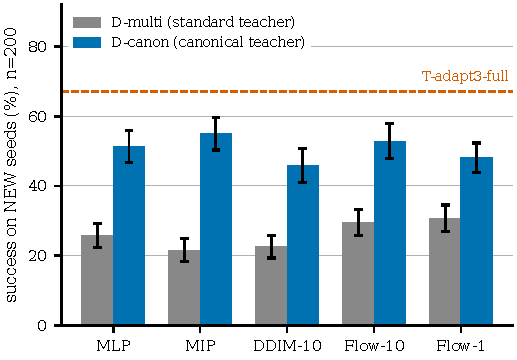
\includegraphics[width=0.5\textwidth]{fig_k4}
\caption{Five students trained on data from the standard multimodal teacher (D-multi) or the canonical teacher (D-canon), NEW seeds ($n{=}200$), mean over three training seeds, 95\% CI. The dashed line is T-adapt3-full on the same seeds.}
\label{fig:k4}
\end{figure}

Canonicalising the teacher raised each student by: MLP 25.7\pp\ [19.8, 31.5], MIP 33.5\pp\ [28.0, 38.8], DDIM-10 23.3\pp\ [17.7, 29.0], flow-10 23.3\pp\ [17.3, 29.2], flow-1 17.5\pp\ [11.7, 23.5]. On D-multi, the differences from the MLP are flow-1 +5.0 [$-0.3$, 10.2], flow-10 +3.8 [$-1.0$, 8.7], diffusion $-3.2$ [$-7.7$, 1.3] and MIP $-4.2$ [$-8.8$, 0.5]. The canonical oracle teacher reaches 96.0\% [93.0, 98.5] and T-adapt3-full 67.0\% [60.5, 73.5], so the best D-canon student (MIP, 55.0\%) is $-12.0$\pp\ [$-19.8$, $-4.0$] below it (best student chosen on the same final episodes, which is optimistic for the learned side); all D-multi students are 36.3--45.5\pp\ below. In the earlier privileged-teacher study (NEW $n{=}200$), the canonical oracle reached 92.5\%, T-adapt3-full 60.0\% and the students 58.0--59.5\%. Seed-to-seed spread was 5--15\pp. The data are NEW only, behaviour cloning only (no DAgger) and one data scale (400 scenarios).

\section{Breadth: Other Tasks and Classical Pilots}
\label{app:breadth}

\textbf{Residual PPO on catch, toss and Push-T.} Table~\ref{tab:16a} gives the mini-comparisons (rules in a spike README, order not provable from git; breadth only). Catch and Push-T ties are at the ceiling, where a +10\pp\ win is arithmetically impossible, and toss is uninterpretable because its gate failed four times (best +1.3\pp). Local and remote runs of 30 episodes had identical outcomes, lengths and joint trajectories; the only difference was 7.8e-16 in a Push-T summary statistic.

\begin{table}[htbp]
\centering
\caption{Residual PPO on the CAL-tuned strongest classical, learned minus classical (pp [95\% CI]).}
\label{tab:16a}
\begin{tabular}{@{}lllllll@{}}
\toprule
Task & Gate (pp) & Classical HOLD / NEW & HOLD ($n{=}500$) & NEW ($n{=}200$) & Verdict \\ \midrule
Catch & +54.0 [48.3, 59.7] & 0.992 / 1.000 & $-0.5$ [$-1.1$, 0.1] & $-0.7$ [$-1.8$, 0.0] & tie (ceiling) \\
Push-T & +61.3 (1 seed) & 0.990 / 0.995 & +0.4 [$-0.4$, 1.2] & $-1.5$ [$-3.5$, 0.0] & tie (ceiling) \\
Toss & failed 4 times & 0.680 / 0.685 & +0.6 [$-1.2$, 2.4] & $-1.0$ [$-3.0$, 1.0] & no verdict \\
\bottomrule
\end{tabular}
\end{table}

\textbf{Classical pilots (demo seeds, no learned comparison).} On the tracking ladder ($n{=}5$) the RMSE is 0.0074 (PID), 0.0061 (CTC+LQR), 0.0056 (iLQR), 0.0056 (iLQR-MPC) and 0.0073 (MPPI) rad. Catching succeeds 19 of 20 without error but 6 of 20 with 10\,ms ball-position delay; whip with a chain 10\% shorter succeeds 12 of 20; Push-T succeeds 19 of 20 with 20\,ms sensor delay and 0 of 20 with 30\,ms. These pilots motivated choosing whip and are not paper claims. An MJX-trained PPO reproduced the CPU PPO within CI with 4.7e6 steps/s on 4096 environments; this engineering result is not used for K1--K4.


\end{document}
